\chapter{Reference Manual}
\label{chpt:Reference}
\typeout{$Id$}

\section{Database Structure}

Each card uses string of up to 36 characters as a unique key.
Cards are indexed by key, title, author, and subject. The keys, titles,
authors, and subjects are always compared in a case-insensitive
fashion.  That is, {\tt "The Door Into Summer"} is the same as {\tt
"THE DOOR INTO SUMMER"}.  Internally, the keys, titles, authors, and
subjects are converted to all uppercase letters.  There is also a
keyword table that associates keywords (search terms) with each card.

\begin{table}[hpt]
\begin{tabular}{|l|l|p{3in}|}
\hline
Name&Type&Description \\
\hline
Key&CHAR(36)&Unique key identifying the item. This is an arbitrary
identifier and could be a LC catalog code or some other user-defined
identifier.  Each card has a unique value for this field.\\
Title&CHAR(128)&The title or name of the item.\\
Author&CHAR(64)&The author of the item. This could be the name of the
performer for audio CDs.\\
Subject&CHAR(128)&The subject of the item.  What this item is generally
about. \\
Description&TEXT&The description of the item.  This is unstructured text
and can be whatever you want.\\
Location&CHAR(36)&The location of the item. This is generally used to
note the physical location of the item, such as a particular book self
or the fact that it is out on loan, etc.\\
Category&CHAR(36)&The category of the item. Some user defined category.\\
Media&CHAR(36)&The media the item is on. The type of media of the item,
such as hardbound book, or audio CD.\\
Publisher&CHAR(36)&The publisher of the item. The publisher or producer
of the item.\\
PubLocation&CHAR(36)&The location of the publisher. The publisher's
location (usually just the city).\\
PubDate&DATE&The date the item was published. The publication date.\\
Edition&CHAR(36)&The edition of the item. Whether this is a first
edition or a second edition, etc.\\
ISBN&CHAR(20)&The ISBN of the item. If the item has one.\\
\hline
\end{tabular}
\caption{Data fields in the ``Card'' table.}
\label{tab:ref:cardfields}
\end{table}
Each card contains thirteen (13) pieces of data as shown in
Table~\ref{tab:ref:cardfields}. The keyword table consists of two data
fields, a 64 character keyword and a 36 character card key.

\section{Main GUI Window}

\begin{figure}[hpt]
\begin{centering}
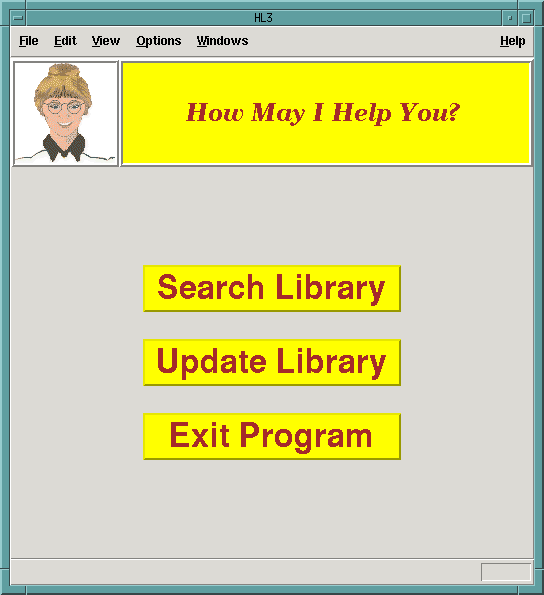
\includegraphics[width=5in]{MainWindow.png}
\caption{The main window of the Home Librarian application}
\label{fig:ref:MainWindow}
\end{centering}
\end{figure}
\begin{figure}[hpt]
\begin{centering}
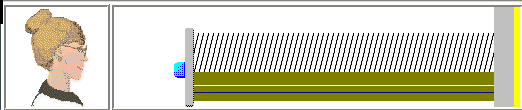
\includegraphics[width=5in]{CardCatDrawer.png}
\caption{Card Catelog Drawer}
\label{fig:ref:headerAnimation}
\end{centering}
\end{figure}
The main window of the Home Librarian application, as shown in
Figure~\ref{fig:ref:MainWindow}, has a progress and status section at
the top of the GUI\footnote{Below the attached menu bar.}, consisting
of a ``face'' area and a progress and status area. The face area holds
either a forward facing librarian image, when the GUI is idle and
waiting for user input or a right profile when the application is
working and not accepting input from the user. The status and progress
either holds the message ``How May I Help You?'' or some sort of status
message, usually detailing the number of matches found when searching,
when the application is idle. When the application is working an
animation of a card catalog drawer being opened and flipped through is
displayed, as shown in Figure~\ref{fig:ref:headerAnimation}.

\begin{figure}[hpt]
\begin{centering}
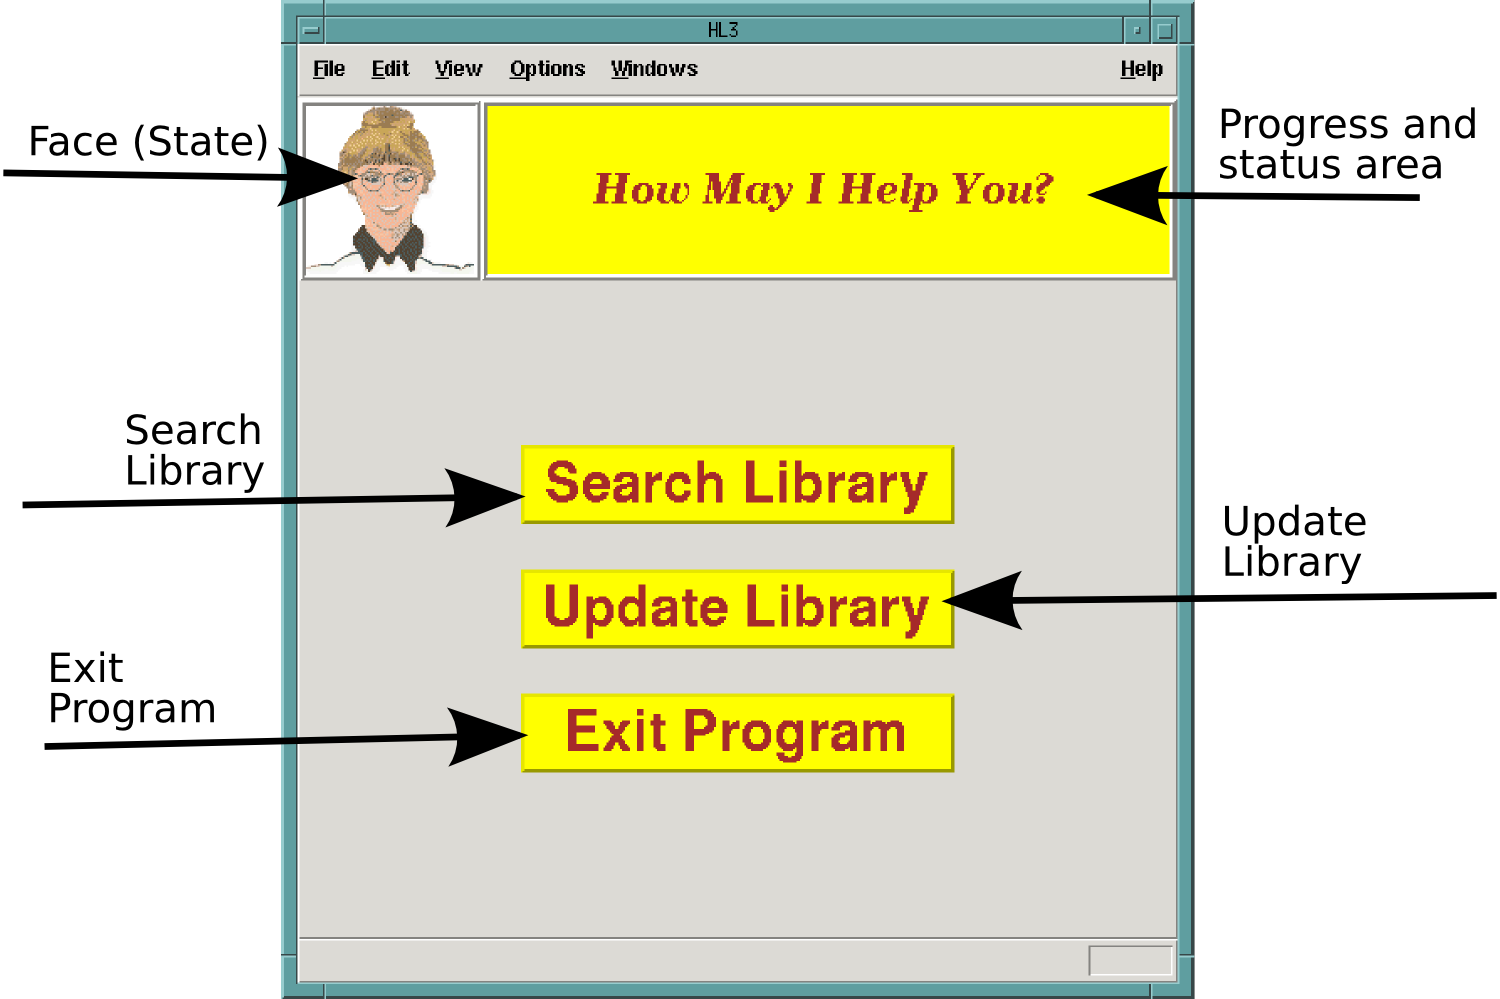
\includegraphics[width=5in]{MainWindowAnnotated.png}
\caption{Main Window, annotated.}
\label{fig:ref:mainwindowAnno}
\end{centering}
\end{figure}
Below the progress and status section is the main interaction area.
Initialially, this contains three big buttons giving access to the major
functions of the application, as shown in
Figure~\ref{fig:ref:mainwindowAnno}. 

\subsection{Buttons on the main window}

There are two main functions supplied by the application: searching a
card catalog database, described in Section~\ref{sect:ref:search} and
editing a card catalog database, described in
Section~\ref{sect:ref:update}. The top most button in the initial (and
idle) state of the main GUI selects the searching function. The next
button selects the editing (update) function. The bottom button exits
the application. All of these operations are available from the File
menu item as well, along with some additional operations.

\section{Searching a database (card catalog)}
\label{sect:ref:search}

\begin{figure}[hpt]
\begin{centering}
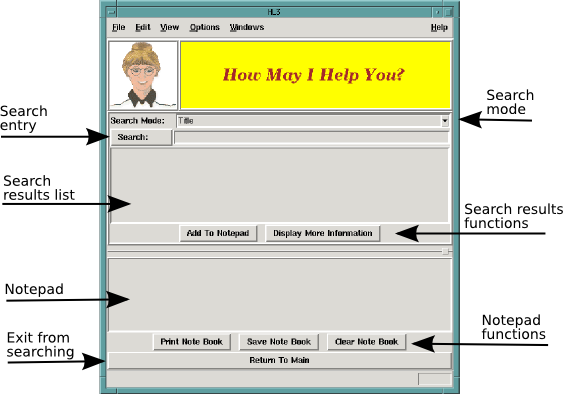
\includegraphics[width=5in]{SearchWindowAnnotated.png}
\caption{Search Window, annotated.}
\label{fig:ref:searchwindowAnno}
\end{centering}
\end{figure}
The Search function version of the Main GUI Window is shown in
Figure~\ref{fig:ref:searchwindowAnno}. This version of the main window
has a dropdown menu to select the search mode, a place for entering a
search string, a search results list box, a set of search results
disposition buttons, a notepad (text) area for making notes, and a set
of buttons to manage the notepad area. 

\subsection{Types of searches}
\label{sect:ref:searchtypes}

There are four types of searches, by title, by author, by subject, and
by keyword. The search strings are considered SQL ``LIKE'' patterns. 
Like patterns use two wildcard characters: ``\%'', which matches any
zero or more characters and ``\_'' which matches exactly one character. 
The four search fields are stored in the database as all uppercase and
the search string is itself converted to upper case, so the search is
always performed in a case insensitive manor. 

\subsection{Search results and what to do with them}

The search results are displayed as a list below the search string. 
These list elements can be selected and either added to the notepad
area (and then printed or saved as a text file) or more information
(the complete card record) can be requested.  

\subsection{The notepad area}

The notepad area below the search results can be used to save selected
result items and its contents can be printed, saved as a text file, or
cleared.

\section{Updating a database (card catelog)}
\label{sect:ref:update}

\begin{figure}[hpt]
\begin{centering}
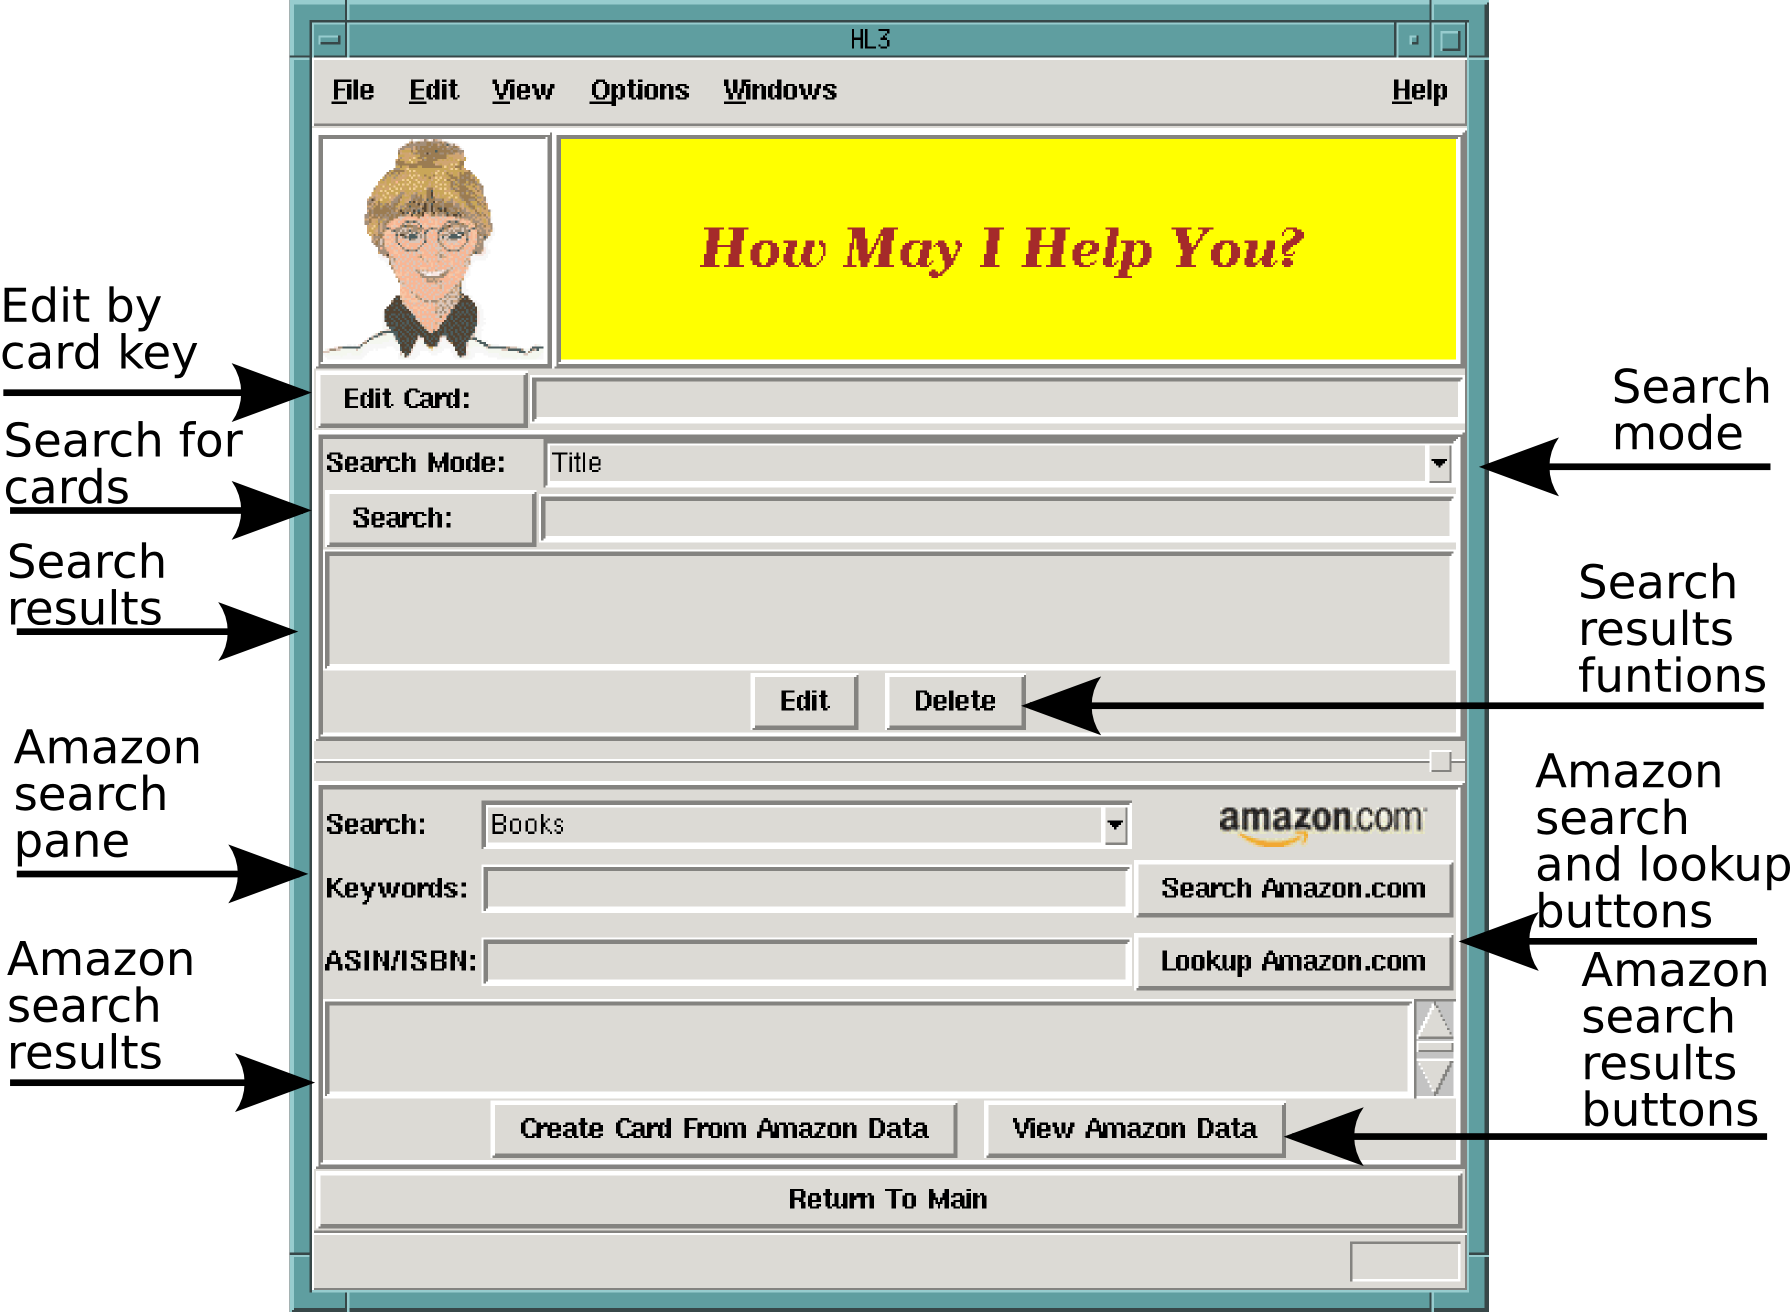
\includegraphics[width=5in]{UpdateWindowAnnotated.png}
\caption{Update Window, annotated.}
\label{fig:ref:updatewindowAnno}
\end{centering}
\end{figure}
The Update function version of the Main GUI Window is shown in
Figure~\ref{fig:ref:updatewindowAnno}.  This version of the main window
has a place to enter a card key to edit, a dropdown menu to select the
search mode, a place for entering a search string, a search results
list box, a set of search results disposition buttons, and an Amazon search
pane to get Amazon information about items in your library.

\subsection{Editing a card by its key}
Entering a card key and clicking on \verb=Edit Card= will edit either
an existing card (if the key is in use) or create a new card (if the
key is not in use). The card editor window is shown in
Figure~\ref{fig:ref:editcardAnno}. If this is a new card, the ``Get New
Card Template Or Amazon URL Dialog'', described in
Section~\ref{sect:ref:newcardtempl} is displayed. See
Section~\ref{sect:ref:editcard} for more information about the card
editor window.

\subsection{Editing a card by searching for it}
A search can be performed to find a card to edit. The searching is much
the same as described in Section~\ref{sect:ref:searchtypes}. Cards found
by searching can be either edited or deleted.

\subsection{Searching Amazon's database}

Amazon's huge database of books, audio tapes, CDs, video tapes, and
DVDs can be searched with the lower half of the update window.  Result
elements can be used to create new cards or used to provide information
for existing cards.  Amazon's database can be searched  entering search
terms and selecting what type of items to look for, this includes
books, music, video, CDs, and DVDs.  It is also possible to use an ISBN
or ASIN to look up a specific item.  The search results are listed below
the search entries and these items can be selected and used to create a
new card or to just view the information in a new window (see
Section~\ref{sect:ref:viewamazondata}).

\section{Dialog Boxes}
\subsection{Get Connection String Dialog}
\label{sect:ref:getconnectionstring}
This dialog box creates the connection string needed to connect to the
database via the ODBC API. The dialog shows lists of the available
drivers and available datasources.  Either a datasource can be used
directly or a connection string can be created from an available
driver. One of the possible configuration files can be used to store
the connection string for future invocations of the Home Librarian
program.
\subsection{Select A Template Dialog}
This dialog box selects a template card.
\subsection{Edit Template}
This window edits a template card.
\subsection{Edit Card}
\label{sect:ref:editcard}
\begin{figure}[hpt]
\begin{centering}
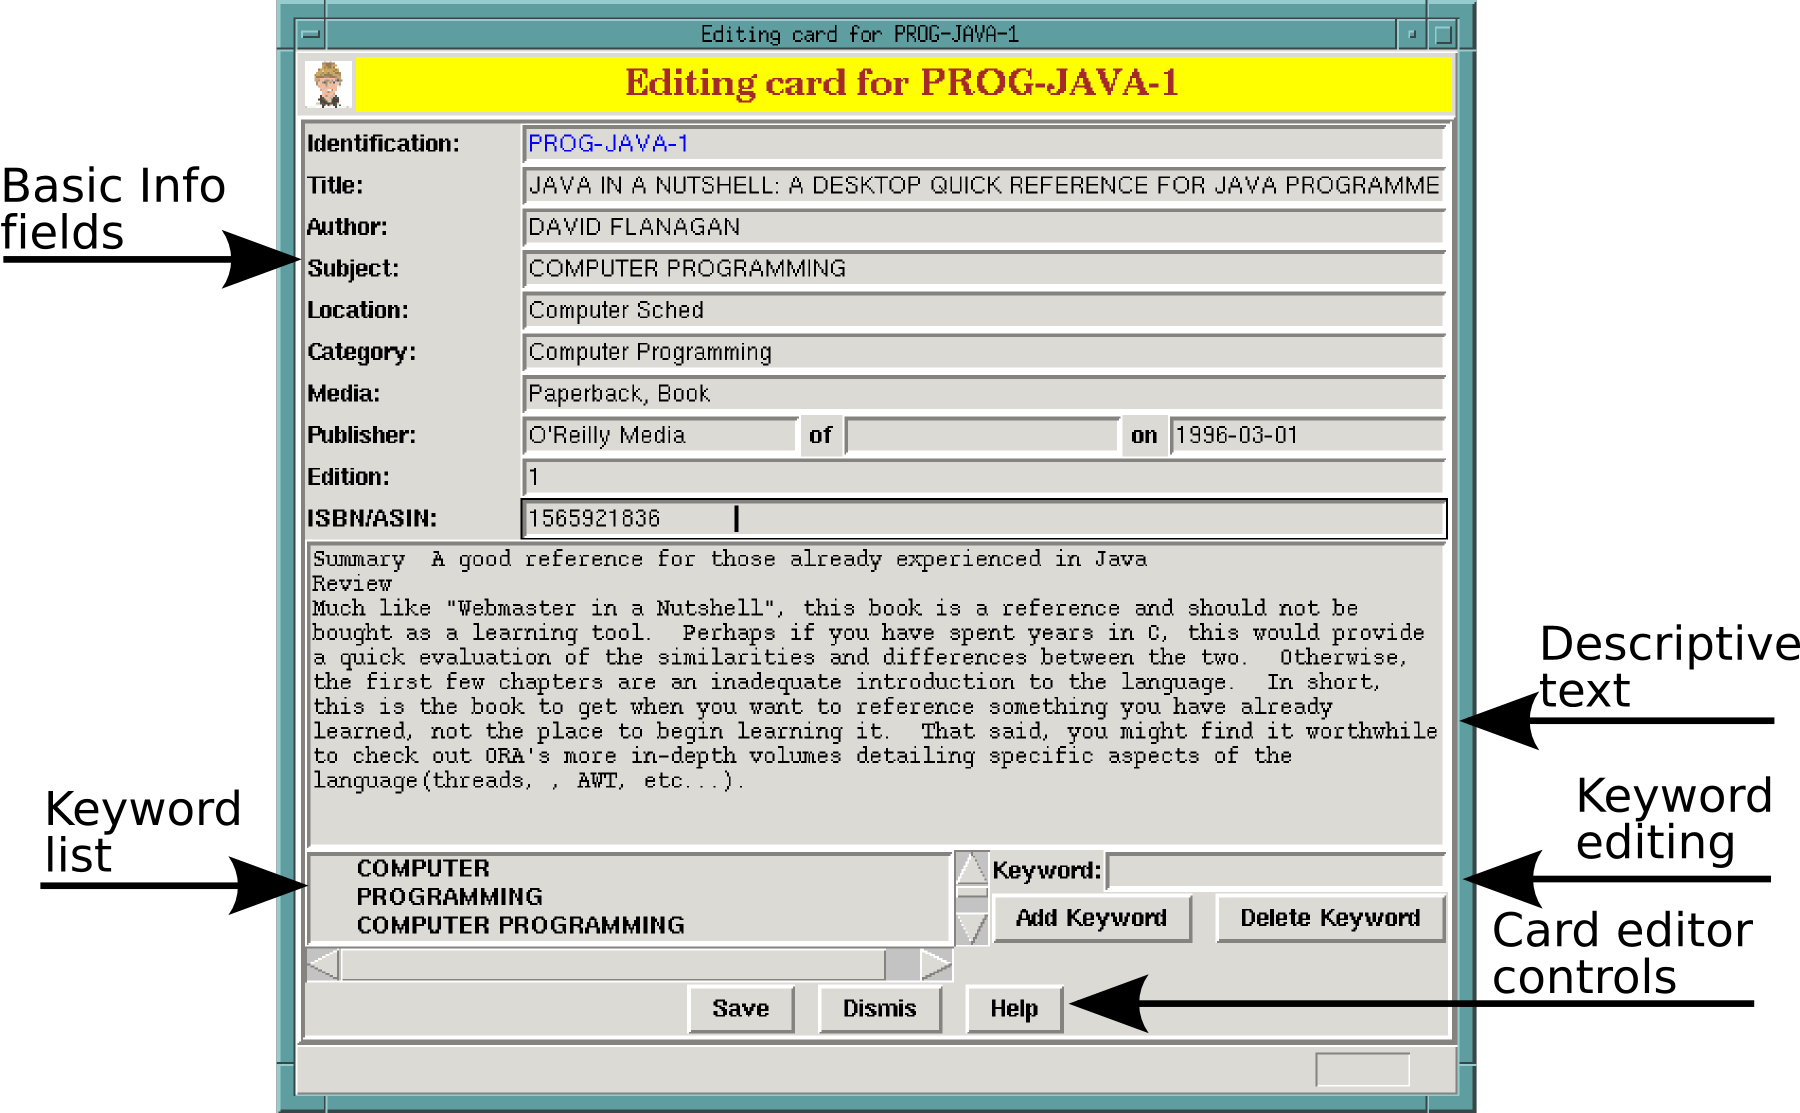
\includegraphics[width=5in]{EditCardAnnotated.png}
\caption{Edit Card Window, annotated.}
\label{fig:ref:editcardAnno}
\end{centering}
\end{figure}
The card editor window, shown in Figure~\ref{fig:ref:editcardAnno},
contains a collection of basic informational fields in its upper
section, with a field containing descriptive text.  Near the bottom is
a section containing the keywords associated with this card, along with
a set of controls for adding and deleting keywords.  At the very bottom
are buttons for saving the card, dismissing the card editor, and for
getting help.

The short fields in the upper section are a standard collection of
information fields, including the card identifcation (its unique key),
title, the author, the subject, the location, the category, the media,
the publisher, the edition, and the ISBN or ASIN of the item.  Except
for the identifcation field, all of the fields can be edited.  The
title, author, and subject fields are converted to all upper case
letters for easy searching. The descriptive text is free form text that
describes the item. The keywords can be any usefull search terms of
your choosing. Keywords can be added or deleted.  The keywords are
converted to all uppercase letters for easy searching.

\subsection{Get New Key Dialog}
This dialog box gets a new key.
\subsection{Get New Card Template Or Amazon URL Dialog}
\label{sect:ref:newcardtempl}
This dialog selects either a template or gets data from Amazon to initialize 
a new card.
\subsection{Import Dialog}
This dialog box selects a file and mode for data import.
\subsection{Select Printer Dialog}
This dialog box is used to select a printer or Postscript output file.
The print format and other output details are also selected with this
dialog box.
\subsection{Select A Layout Dialog}
This dialog box selects a print layout, either from the layout cache or
from a disk file.
\subsection{Edit Layout Text Tool Dialog}
This tool dialog box is used to create a text item in a card layout.
\subsection{Edit Layout Line Tool Dialog}
This tool dialog box is used to create a line item in a card layout.
\subsection{Edit Layout Rect Disk Tool Dialog}
This tool dialog box is used to create a rectangle or disk item in a
card layout.
\subsection{Edit Layout Bitmap Tool Dialog}
This tool dialog box is used to create a bitmap item in a card layout.
\subsection{Edit Layout Resize Tool Dialog}
This tool dialog box is used to resize an existing item in a card layout.
\subsection{Edit Layout}
This window provides for editing a card layout.
\subsection{Print Progress}
This window shows the print progress of either text output or cards.
\subsection{More Info Window}
This window shows more information about a selected card.
\subsection{View Amazon Data}
\label{sect:ref:viewamazondata}

